
\newpage
\thispagestyle{empty}
\mbox{}
\setlength{\parskip}{4mm}
\chapter{Algoritmos de Localización}
\label{ch:chapter2}


Todos los sistemas a continuación serán descritos desde el punto de vista de sistemas en variables de estado. Para los modelos utilizados los vehículos se interpretan como masas puntuales en el espacio centrados en el centro de masa de estos. Con esto en consideración se puede pasar.

\section{Descripción de un vehículo como modelo continuo}
\par
Considerando que los vehículos autónomos tienen como entrada su velocidad y se puede cuantificar su magnitud en el eje X e Y con lo que la evolución de la posición del vehículo en este eje de coordenadas es descrita con el siguiente sistema. 
\begin{equation*}
\left.
 \begin{aligned}
P_{x_1}(t) & = P_{x_1}(0)+V_{x_1}(t)\cdot t \\
P_{y_1}(t) & = P_{y_1}(0)+V_{y_1}(t)\cdot t
\end{aligned}
\right\}
\quad\text{Sistema de un vehiculo continuo}
\end{equation*}
\par
Esto es considerando que se esta tratando con un sistema continuo, sin embargo, al tratarse de sistemas digitales este modelo deja de ser válido y se tendrá que pasar al siguiente. 
\begin{equation*}
\left.
 \begin{aligned}
P_{x_1}(k+1) & = P_{x_1}(k)+V_{x_1}(k)\cdot\Delta{T} \\
P_{y_1}(k+1) & = P_{y_1}(k)+V_{y_1}(k)\cdot\Delta{T} 
\end{aligned}
\right\}
\quad\text{Sistema de un vehículo discreto}
\end{equation*}
\par
En este sistema se tendrá como estado $q(k)=[P_{x1},P_{y1}]$ lo que implicará que la matriz F simplemente será la matriz identidad. Las entradas del sistema a su vez serán $u(k)=[V_{x1},V_{y1}]$.
No se discutirá todavía sobre la matriz H, esto se tratará en el apartado de corrección de la medida. 
Ahora se tendrá que tomar en consideración la incertidumbre de todos los componentes del sistema. Debido a que los instrumentos de medida tienen una determinada precisión no se podrá conocer con exactitud ni la posición, ni la velocidad del vehículo. Esto puede dar lugar a que el sistema antes descrito llegue a alejarse considerablemente de la realidad. 
\par
Para tomar esto en consideración se sustituirán los estados por elegidos por distribuciones gausianas cuya media corresponderá con la posición estimada del vehículo y la varianza nos dará información de con que probabilidad estará el vehículo dentro de una determinada región. De tal forma que la posición y velocidad real del vehículo seguirán la siguiente distribución. 
\begin{equation*}
\left.
 \begin{aligned}
P_{x_1}(x) & = \frac{1}{\sigma\sqrt{2\pi}} 
  \exp\left( -\frac{1}{2}\left(\frac{x-\hat{P_{x_1}}}{\sigma}\right)^{\!2}\,\right) \\
P_{y_1}(y) & = \frac{1}{\sigma\sqrt{2\pi}} 
  \exp\left( -\frac{1}{2}\left(\frac{y-\hat{P_{y_1}}}{\sigma}\right)^{\!2}\,\right)
\end{aligned}
\right\}
\quad\text{Distribución de la posición de un vehículo}
\end{equation*}

\begin{equation*}
\left.
 \begin{aligned}
V_{x_1}(x) & = \frac{1}{\sigma\sqrt{2\pi}} 
  \exp\left( -\frac{1}{2}\left(\frac{x-\hat{V_{x_1}}}{\sigma}\right)^{\!2}\,\right) \\
V_{y_1}(y) & = \frac{1}{\sigma\sqrt{2\pi}} 
  \exp\left( -\frac{1}{2}\left(\frac{y-\hat{V_{y_1}}}{\sigma}\right)^{\!2}\,\right)
\end{aligned}
\right\}
\quad\text{Distribución de la velocidad de un vehículo}
\end{equation*}

\par
Esto se puede hacer debido a que la suma de dos distribuciones gausianas independientes tiene la propiedad de que la media resultante será $\mu_{x+y}=\mu_{x}+\mu_{y}$ y la varianza $\sigma_{x+y}^2=\sigma_{x}^2+ \sigma_{y}^2$. Esto implica que el sistema seguirá siendo lineal. Se añadirá una matriz adicional que tomara en cuenta la evolución de la incertidumbre de (aumentara con el tiempo) y la media de estas gausianas sustituirán los estados. 
\par
En este punto se hace la distinción entre posición y velocidad real y posición estimada, siendo la posición estimada la que se determina con el sistema anteriormente descrito. Con esto los nuevos estados $\hat{q}(k)=[\hat{P_{x1}},\hat{P_{y1}}]$ y las entradas $\hat{u}(k)=[\hat{V_{x1}},\hat{V_{y1}}]$.
\par
En este punto se puede comparar la trayectoria estimada del vehículo con una de las trayectorias reales posibles que se pueden generar con el modelo utilizado. El primer caso para analizar es tener una posición inicial real diferente a la estimada, es decir que $q(0)\neq\hat{q}(0)$. Como se observa en la siguiente figura esta diferencia no tiene mucha influencia en la posición final del vehículo.  
\par

\begin{figure}[htb]
\centering
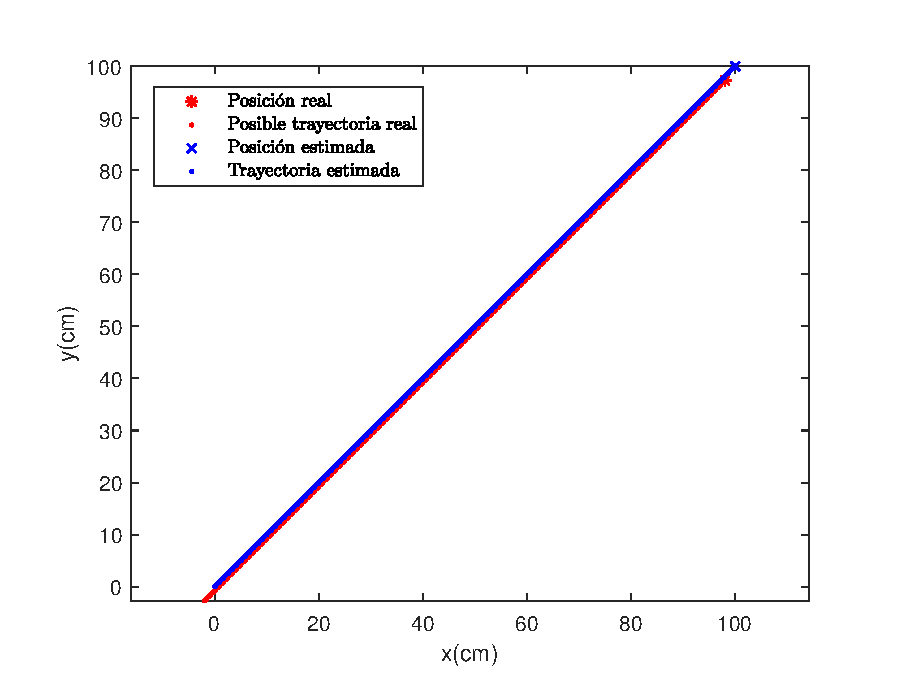
\includegraphics[width=0.8\textwidth]{figures/Figura-de-desviación-de-un-vehiculo-con-posición-incial-deferente-a-la-real.eps}
\caption{Diferencia entre trayectoria estimada y trayectoria real para posiciones iniciales diferentes} \label{fig:Pini_dif}
\end{figure}

Otro caso sencillo por analizar es que ocurre para una entrada constante (velocidad constante) donde $u(0)\neq\hat{u}(0)$.

\begin{figure}[htb]
\centering
\includegraphics[width=0.8\textwidth]{figures/Figura-de-desviación-de-un-vehiculo-con-velocidad-inicial-diferente-a-la-real.eps}
\caption{Diferencia entre trayectoria estimada y trayectoria real para velocidades iniciales diferentes} \label{fig:Vini_dif}
\end{figure}
\par 

En este caso el error es acumulativo y la diferencia entre la posición inicial y la posición final es significativa, por esta razón se debe recurrir a métodos de corrección para tener en consideración este tipo de incertidumbre. 

\section{Corrección utilizando el filtro de Kalman.}
Como se observo en una sección anterior la actualización de la incertidumbre del sistema se toma en cuenta en la matriz P a través de la siguiente expresión 
\begin{equation*}
\left.
 \begin{aligned}
P(k+1)&=FP(k)F'+GQG'
\end{aligned}
\right\}
\end{equation*}
Donde la matriz Q es la matriz de covarianza de la entrada.
\par
En este punto es donde se hará uso de la relación de la salida del sistema de variables de estado con los propios estados del sistema 
\begin{equation*}
\left.
 \begin{aligned}
y(k)&=H\cdot{q(k)}
\end{aligned}
\right.
\end{equation*}
Se llamará H a la matriz de medida. En el caso más sencillo la medida obtenida será $P_{x1}$ y $P_{y1}$ quedando la matriz H como:
\begin{equation*}
\left.
 \begin{aligned}
H=\begin{pmatrix}
1 & 0\\
0 & 1 
\end{pmatrix}
\end{aligned}
\right.
\end{equation*}
Quedando así la salida del sistema estimada como:
\begin{equation*}
\left.
 \begin{aligned}
\hat{y}(k)=\begin{pmatrix}
1 & 0\\
0 & 1 
\end{pmatrix}\begin{pmatrix}
\hat{P_{x1}}\\
\hat{P_{y1}} 
\end{pmatrix}
\end{aligned}
\right.
\end{equation*}
Para realizar la corrección en de los estados se realiza la siguiente operación 
\begin{equation*}
\left.
 \begin{aligned}
\hat{q}(k)&=\hat{q}(k)+K\cdot{(y_{m}-\hat{y}(k))}
\end{aligned}
\right.
\end{equation*}
Siendo $y_{m}$ en este caso $\begin{pmatrix}
P_{x1}\\
P_{y1} 
\end{pmatrix}$, es decir la posición real del objeto, y K la ganancia del filtro de Kalman. 
También utilizando esta misma matriz H se actualiza la matriz de covariaza. 
\begin{equation*}
\left.
 \begin{aligned}
P=P-K·H·P
\end{aligned}
\right.
\end{equation*}
Cabe destacar que como las mediciones no están ligadas de ninguna manera la matriz P será diagonal todo el tiempo y los autovalores de esta matriz definirán los ejes de una elipse centrada en $[\hat{P_{x1}},\hat{P_{y1}}]$. Esta elipse indica el área en el que se puede encontrar el vehículo con un 68\% de probabilidad (una desviación típica). 
\par 

%\begin{figure}[h!]
%\centering
%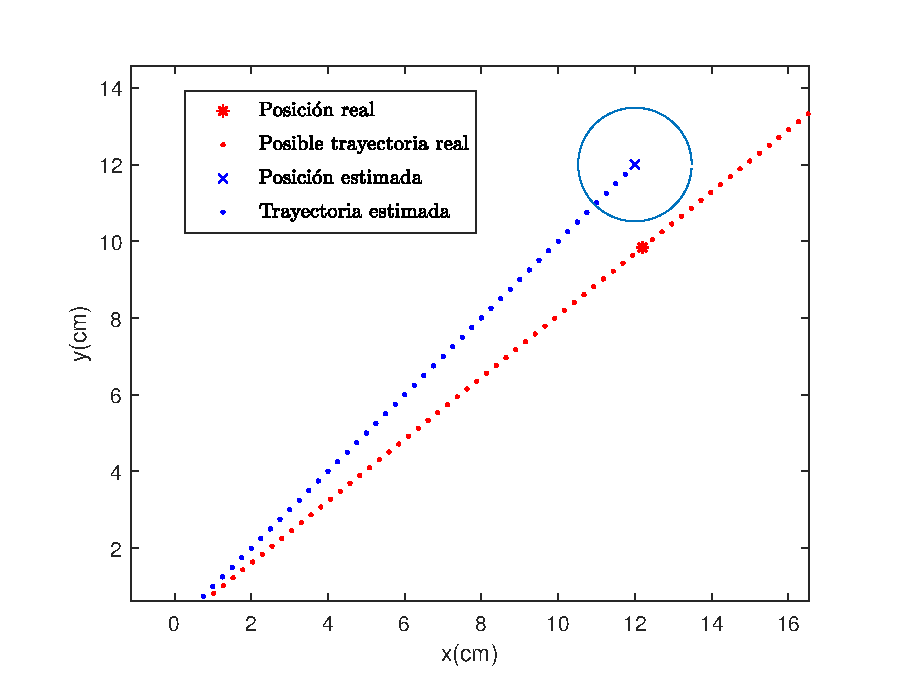
\includegraphics[width=0.8\textwidth]{figures/GraficarUnicarAntesdecorreccion.eps}
%\caption{Estado del sistema previo a una corrección} 
%\label{fig:Unicar_pre}
%\end{figure}
%\par 
%\begin{figure}[h!]
%\centering
%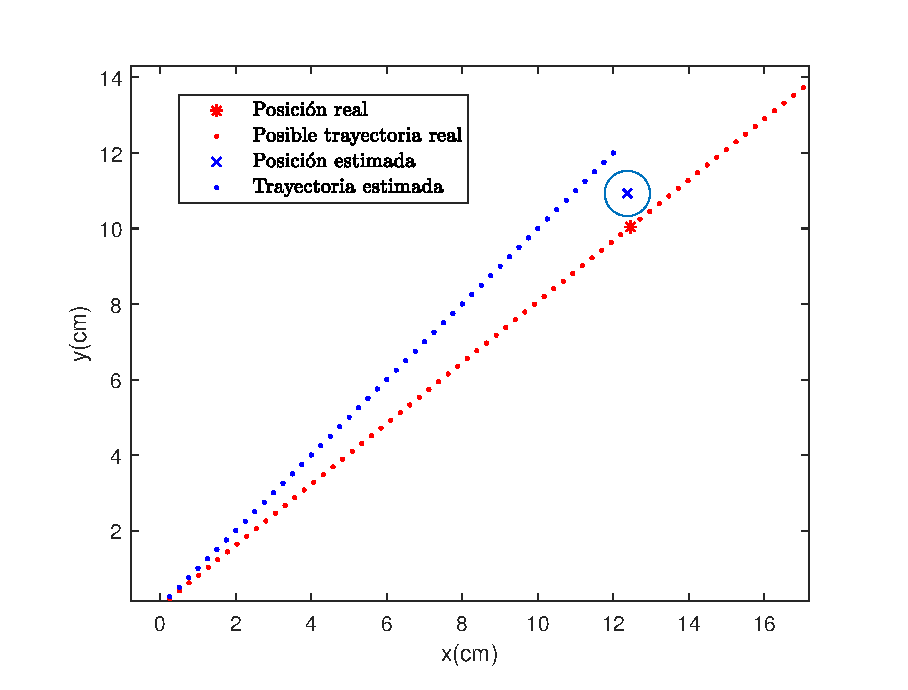
\includegraphics[width=0.8\textwidth]{figures/GraficarUnicardespuescorreccion.eps}
%\caption{Estado del sistema previo a una corrección} 
%\label{fig:Unicar_post}
%\end{figure}
%\par 



Sin embargo, por la restricción de hardware impuestas hacer una corrección individual de la posición global en X e Y no es posible. Únicamente se dispondrán de las distancias entre dos vehículos. Por lo que el sistema mínimo para obtener correcciones son dos vehículos. 
\newpage

\begin{figure}[!htb]
  \begin{center}
    \subfigure[Previo a corrección]{
        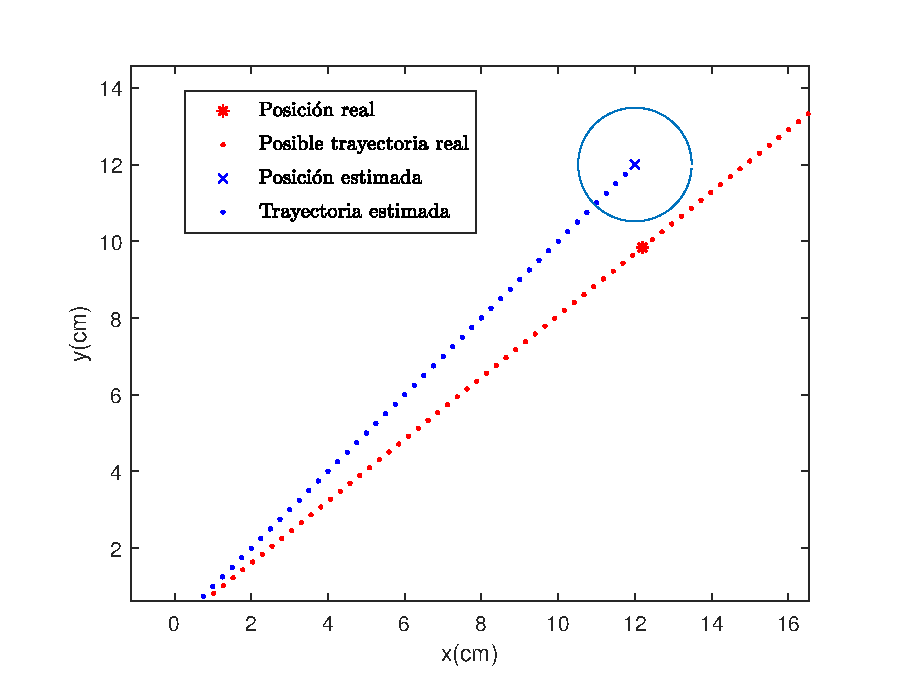
\includegraphics[width=0.7\textwidth]{figures/GraficarUnicarAntesdecorreccion.eps}
        \label{subfig:Unicar_pre}}
    \subfigure[Después corrección]{
        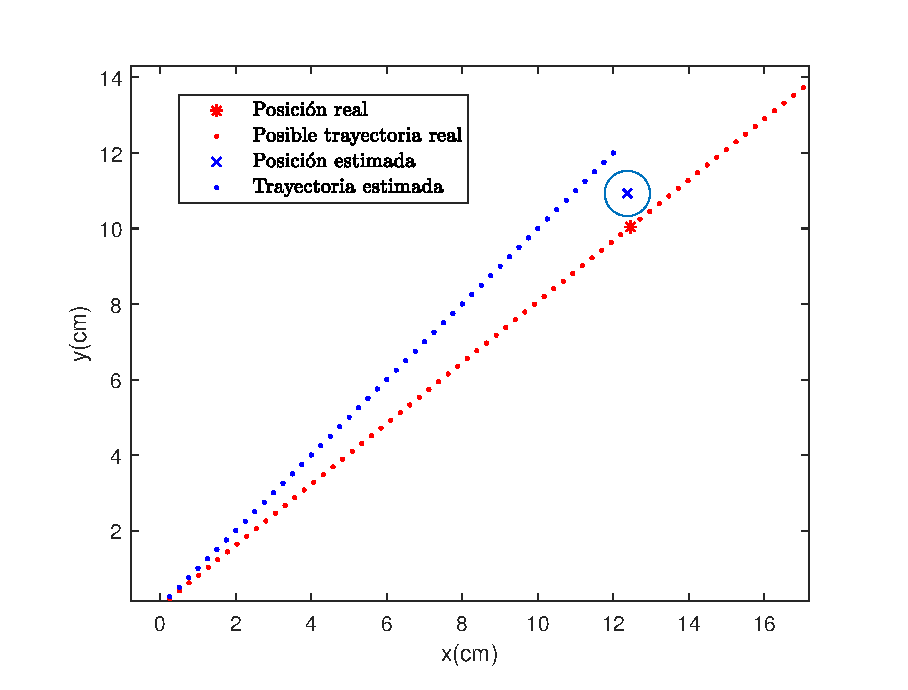
\includegraphics[width=0.7\textwidth]{figures/GraficarUnicardespuescorreccion.eps}
        \label{subfig:Unicar_pos}}
    \caption{Corrección con filtro de Kalman:Antes y después}
    \label{fig:CorrciónUnicar}
  \end{center}
\end{figure}
\newpage

\section{Extensión a dos vehículos}
El sistema de dos vehículos es una simple extensión del sistema de 1 vehículo

\begin{equation*}
\left.
 \begin{aligned}
P_{x_1}(k+1) & = P_{x_1}(k)+V_{x_1}(k)\cdot\Delta{T} (1) \\
P_{y_1}(k+1) & = P_{y_1}(k)+V_{y_1}(k)\cdot\Delta{T} (2)\\
P_{x_2}(k+1) & = P_{x_2}(k)+V_{x_2}(k)\cdot\Delta{T} (3)\\
P_{y_2}(k+1) & = P_{y_2}(k)+V_{y_2}(k)\cdot\Delta{T} (4)
\end{aligned}
\right\}
\quad\text{Sistema de dos vehiculos}
\end{equation*}
\par
Sin embargo al tener distancias la corrección se tiene que hacer en coordenadas relativas respecto a uno de los vehículos. Eligiendo que el punto de referencia es el vehículo 1 se consigue el sistema en coordenadas relativas simplemente restando la ecuación (1) a la (3) y la ecuación (2) a la (4) obteniendo:

\begin{equation*}
\left.
 \begin{aligned}
P_{x_21}(k+1) & = P_{x_21}(k)+V_{x_21}(k)\cdot\Delta{T} \\
P_{y_21}(k+1) & = P_{y_21}(k)+V_{y_21}(k)\cdot\Delta{T} 
\end{aligned}
\right\}
\quad\text{Sistema de un vehículo discreto}
\end{equation*}
\par
Se elige unas velocidades arbitrarias y se simulan ambos sistemas obteniéndose la figura \ref{fig:2CarAbs-Rel}. Cabe destacar que en este punto todavía no se consideran incertidumbres, solo se compara la evolución del sistema pasando de un eje de coordenadas a otro.
\par 
Ahora tomando en consideración que se trabaja con distribuciones y restas de distribuciones gausianas las incertidumbres del sistema pasaran a ser $\sigma_{21}^2=\sigma_{1}^2+\sigma_{2}^2$. Esto afectara la evolución de la matriz de covarianza P y por ende se traducirá en que se tendrá una mayor incertidumbre de donde estará un vehículo respecto al otro. 
\newpage
\begin{figure}[htb]
\centering
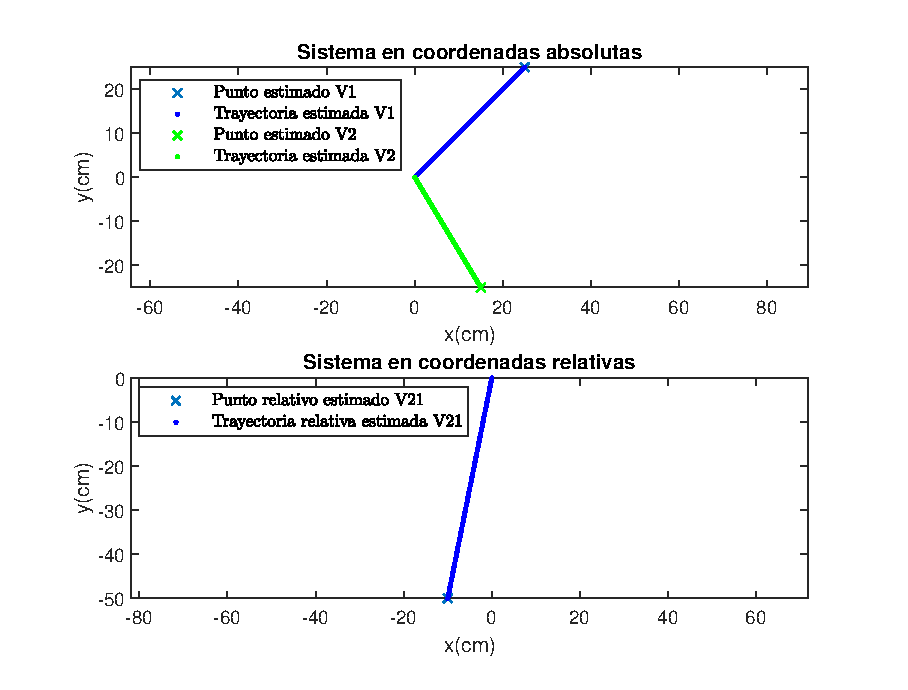
\includegraphics[width=0.8\textwidth]{figures/Sistema2CarAbs-Rel.eps}
\caption{Comparación de sistema en coordenas absolutas frente a relativas} 
\label{fig:2CarAbs-Rel}
\end{figure}
\par 

Ahora tomando en consideración que se trabaja con distribuciones y restas de distribuciones gausianas las incertidumbres del sistema pasaran a ser $\sigma_{21}^2=\sigma_{1}^2+\sigma_{2}^2$. Esto afectara la evolución de la matriz de covarianza P y por ende se traducirá en que se tendrá una mayor incertidumbre de donde estará un vehículo respecto al otro. 
\par
Una vez establecido el sistema en coordenadas relativas se puede realizar la corrección con la distancia. Hacer la corrección con la distancia tendrá dos implicaciones.
\begin{itemize}
	\item Al ser una combinación de la posición relativa en X y en Y (estados $\hat{P_{x_{21}}}$ y $\hat{P_{y_{21}}}$) al realizar la corrección estos estados estarán ligados por lo que la matriz P dejara de ser diagonal. 
	\item Es una combinación no lineal de los estados por lo que la matriz H se tendrá que ajustar a este hecho. 
\end{itemize}
Por último, hacer una corrección con una sola distancia presenta ambigüedad puesto a que si el segundo se encuentra en cualquier posición dentro del círculo de radio $d_{21}$, se detectara como que la trayectoria estimada es correcta a pesar de que el vehículo se puede estar desplazando en una dirección opuesta a la trayectoria real. 

\begin{figure}[htb]
\centering
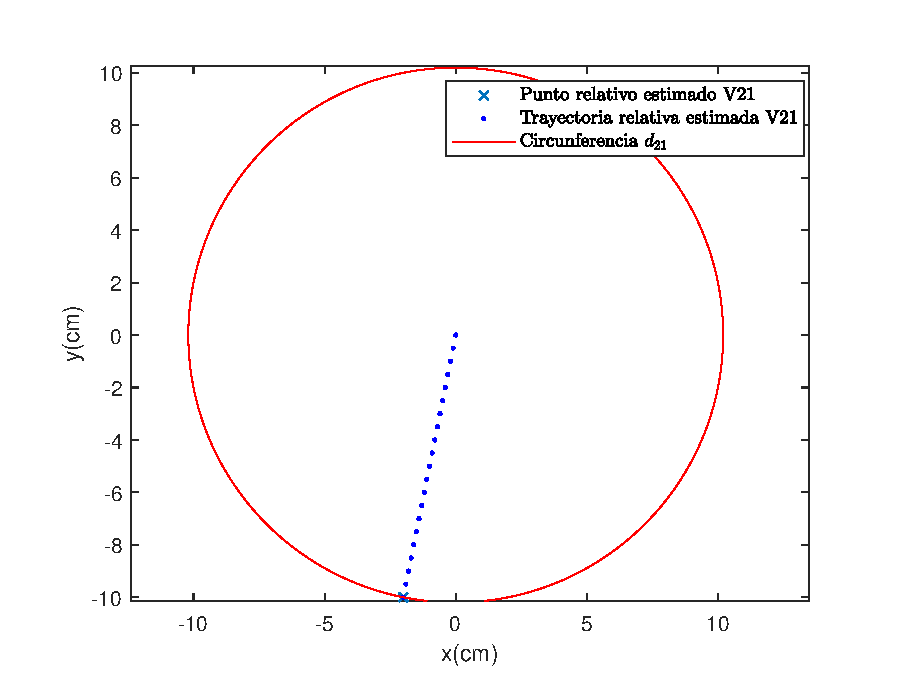
\includegraphics[width=0.8\textwidth]{figures/RadioAmbiguedad.eps}
\caption{Circunferencia correspondiente a $d_{21}$} 
\label{fig:Ambiguedad_1d}
\end{figure}
\par 

En la figura \ref{fig:Ambiguedad_1d} se muestra todos los puntos que tendrán una salida igual utilizando la matriz H discutida anteriormente. Ahora si se plantea un caso posible donde la velocidad real del vehículo difiere de la velocidad estimada de tal manera que la distancia sea la misma para ambas se podrá observar la consecuencia de solo tener una corrección con solo una medida de distancia \ref{fig:Corrción2car}. 

\begin{figure}[!htb]
  \begin{center}
    \subfigure[Previo a corrección]{
        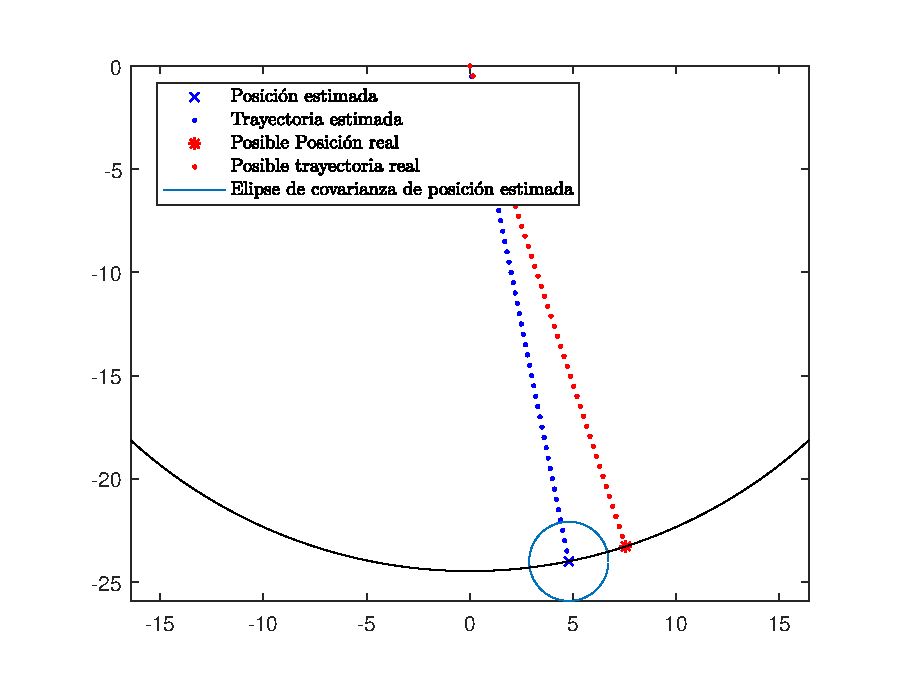
\includegraphics[width=0.7\textwidth]{figures/AmbiguedadPrecorreccion.eps}
        \label{subfig:2car_pre}}
    \subfigure[Después corrección]{
        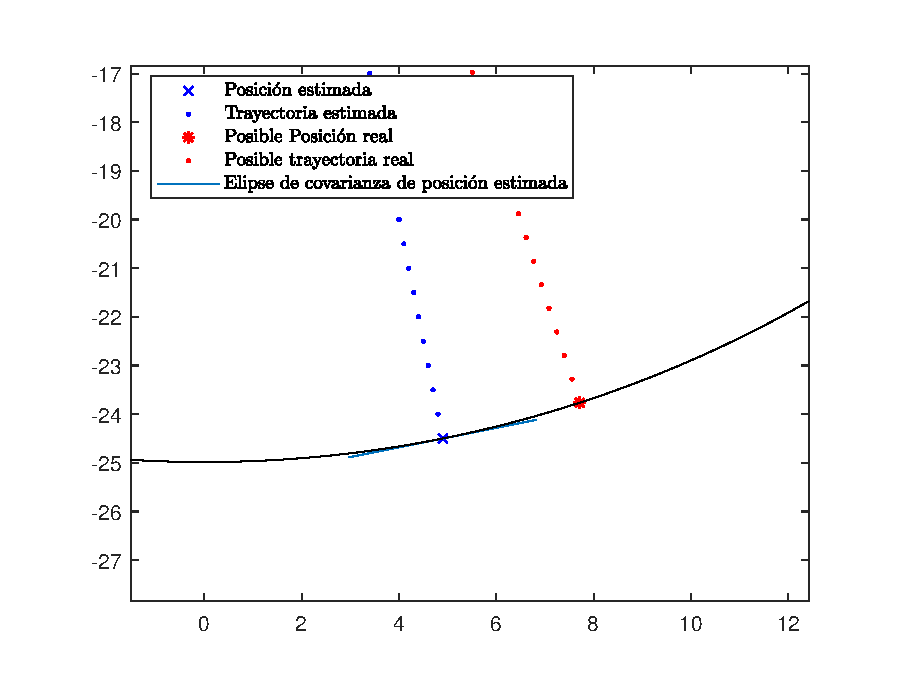
\includegraphics[width=0.7\textwidth]{figures/AmbiguedadPostcorreccion.eps}
        \label{subfig:2car_pos}}
    \caption{Corrección con filtro de Kalman:Antes y después}
    \label{fig:Corrción2car}
  \end{center}
\end{figure}